
%% bare_jrnl.tex
%% V1.4
%% 2012/12/27
%% by Michael Shell
%% see http://www.michaelshell.org/
%% for current contact information.
%%
%% This is a skeleton file demonstrating the use of IEEEtran.cls
%% (requires IEEEtran.cls version 1.8 or later) with an IEEE journal paper.
%%
%% Support sites:
%% http://www.michaelshell.org/tex/ieeetran/
%% http://www.ctan.org/tex-archive/macros/latex/contrib/IEEEtran/
%% and
%% http://www.ieee.org/


\documentclass[journal]{IEEEtran}

\usepackage[utf8]{inputenc}
\usepackage[T1]{fontenc}
\usepackage{lmodern} % load a font with all the characters

\usepackage[style=numeric-comp,backend=biber,url=false]{biblatex}
\addbibresource{bibliography.bib}

\usepackage{cleveref}


% *** GRAPHICS RELATED PACKAGES ***
\usepackage[pdftex]{graphicx}
\graphicspath{{figures/}}
\DeclareGraphicsExtensions{.pdf,.jpg,.png}


% *** MATH PACKAGES ***
%
\usepackage[cmex10]{amsmath}
\interdisplaylinepenalty=2500

% correct bad hyphenation here
\hyphenation{}

% Glossaries
\usepackage[acronym,nopostdot,style=super,nonumberlist]{glossaries}
\makeglossaries
\loadglsentries[main]{glossaries}


\usepackage{gensymb}

\begin{document}
\boldmath

\title{Multi-purpose system for measuring electrical power supplied by electric sockets}

\author{Peter~Babič\\% <-this % stops a space
        Department of Theoretical and Industrial Electrical Engineering (DTIEE)\\%
        babicpet@gmail.com%
}

% The paper headers
\markboth{Paper covering Masters thesis, May~2016}%
{}


% make the title area
\maketitle


\begin{abstract}
The paper shows the process of designing, building and programming of an inter-connected electronic system. It starts with explaining the fundamentals of the physics underlining the electronic power measurement process. The main part includes diagrams describing the inner working of the hardware, and later software running on it. The manufactured device is capable of measuring the electric power provided by the electric socket to the appliance and send the measured values over Wi-Fi to the cloud, to be visualised on a custom web server employing a charting library to plot the measured quantities over time.
\end{abstract}

% Note that keywords are not normally used for peerreview papers.
\begin{IEEEkeywords}
electrical, power, socket, system
\end{IEEEkeywords}



\IEEEpeerreviewmaketitle



\section{Introduction}

\IEEEPARstart{T}{he} idea is to invent way of measuring the electrical power and some more related information, preferably in a non-invasive way. The non-invasive way means, that the appliance that is being measured does not require any modifications, for instance in a form of some probe or a man-in-the-middle plug, suggesting an embedded system. When the data are obtained, they are presented to the user, preferably plotted as a quantity over time, not just and actual measurement. Since the solution is going to be multi-purpose, it has to incorporate at least one additional function, than just the measurement. In this case it is going to be the remote power-on/power-off of the appliance. The name of the thesis also suggests, that the final solution has to be compatible with the electrical sockets used in the local region, in this case the European ones. Since the solution is going to be an \textit{embedded system} measuring a \textit{physical quantity}, these two topics are described in following chapters.


\section{Electric power fundamentals} \label{s:el_power}
In general physics terms, power is defined as the rate at which energy is transferred (or transformed). Electric energy in particular, begins as electric potential energy – what we commonly refer to as voltage. When electrons flow through that potential energy, it turns into electric energy. In most useful circuits, that electric energy transforms into some other form of energy. Electric power is measured by combining both how much electric energy is transferred, and how fast that transfer happens.

The electric power P is equal to the energy consumption E divided by the consumption time t \cite{meade2002foundations}
$$P = \frac Et$$
where P is the electric power in watt [W], E is the energy consumption in joule [J] and 
t is the time in seconds [s].

Electrical Power, in a circuit is the amount of energy that is absorbed or produced within the circuit. A source of energy such as a voltage will produce or deliver power while the connected load absorbs it. Light bulbs and heaters for example, absorb electrical power and convert it into heat or light. The higher their value or rating in watts the more power they will consume.

\subsection{Ohm's law}
Ohm's Law deals with the relationship between the voltage and the current in an ideal conductor. This relationship states that: the potential difference (voltage) across an ideal conductor is proportional to the current through it \cite{henry2008ohm}. The constant of proportionality is called the \textit{resistance}.
$$I = \frac U R $$
where I is the current expressed in amperes [A], U is the voltage, bearing the volt units [V] and R is the electrical resistance in ohms [\ohm].

The Ohms's law can be further expanded \cite{beaty1998electric}, to get these three quantities in relationship with \textbf{power}, such as
$$P = I \cdot U = I^2 \cdot R = \frac{U^2}R$$


\subsection{Direct current (DC) circuits}
Generally, Ohm's law is used on \gls{dc} circuits, containing a current of fixed magnitude (amplitude) and a definite direction associated with it. \acrlong{dc} is produced by power supplies, batteries, dynamos and solar cells to name a few.

We also know that \gls{dc} power supplies do not change their value with regards to time\cite{herman2012direct}, they are a constant value flowing in a continuous steady state direction. In other words, \gls{dc} maintains the same value for all times and a constant uni-directional DC supply never changes or becomes negative unless its connections are physically reversed.


\subsection{Waveforms and alternating current (AC) circuits} \label{ss:power_ac}
An alternating function or \gls{ac} waveform on the other hand is defined as one that varies in both magnitude and direction in more or less even manner with respect to time making it a “bi-directional” waveform \cite{whitaker2006ac}. An AC function can represent either a power source or a signal source with the shape of an AC waveform generally following that of a mathematical sinusoid as defined by
$$A(t) = A_{max} \cdot sin(2 \pi f t)$$

\begin{figure}[ht!]
\centering
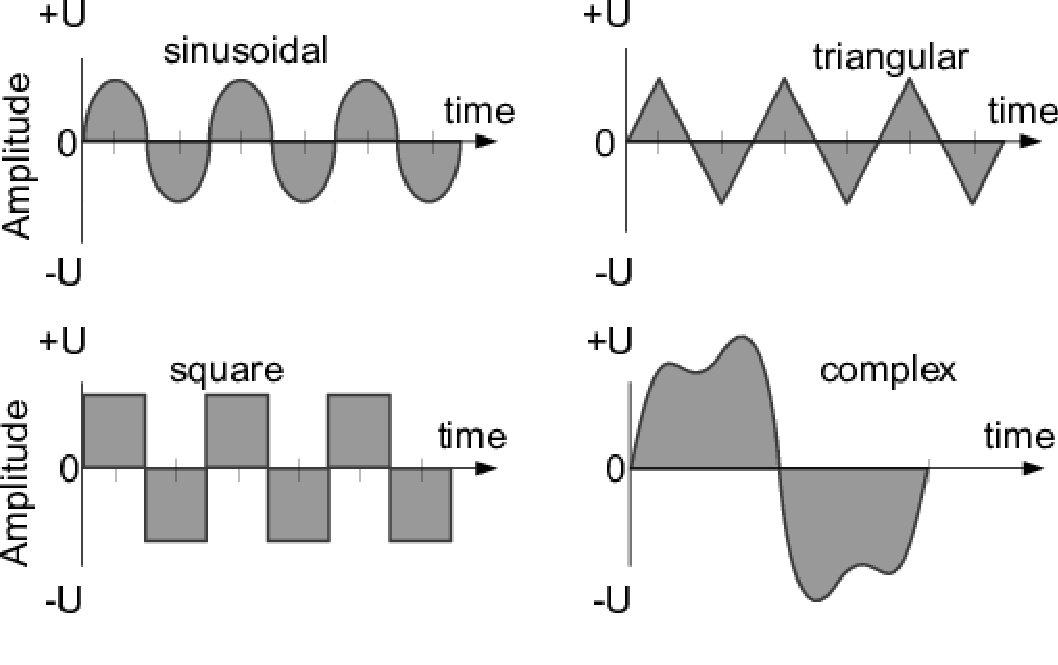
\includegraphics[width=1\linewidth,angle=0]{waveforms}
\caption{The common types of waveforms visualised as a function of amplitude}\label{f:waveforms}
\end{figure}

The term AC or to give it its full description of Alternating Current, generally refers to a time-varying waveform with the most common of all being called a \textbf{Sinusoid} better known as a \textbf{Sinusoidal waveform}. Sinusoidal waveforms are more generally called by their short description as \textbf{Sine Waves}. Sine waves are by far one of the most important types of AC waveform used in electrical engineering.

This means then that the \gls{ac} waveform is a “time-dependent signal” with the most common type of time-dependant signal being that of the Periodic Waveform. The periodic or \gls{ac} waveform is the resulting product of a rotating electrical generator. Generally, the shape of any periodic waveform can be generated using a fundamental frequency and superimposing it with harmonic signals of varying frequencies and amplitudes but that is out of the waveform fundamentals theory.

Alternating voltages and currents can not be stored in batteries or cells like \gls{dc} can, it is much easier and cheaper to generate these quantities using alternators or waveform generators when they are needed. The type and shape of an AC waveform depends upon the generator or device producing them, but all \gls{ac} waveforms consist of a zero voltage line that divides the waveform into two symmetrical halves. The main characteristics of an \gls{ac} waveform \cite{nicolaides1996electrical} are defined as:

\begin{itemize}
\item \textbf{Period (T)} is the length of time in seconds that the waveform takes to repeat itself from start to finish. This can also be called the Periodic Time of the waveform for sine waves, or the Pulse Width for square waves
\item \textbf{Frequency} is the number of times the waveform repeats itself within a one second time period. Frequency is the reciprocal of the time period, defined as $f = \frac 1 T$, with the unit of frequency being the Hertz [Hz]
\item \textbf{Amplitude}  is the magnitude or intensity of the signal waveform 
\end{itemize}


\subsection{Power in AC circuits} \label{ss:ac_power}
When a reactance (either inductive or capacitive) is present in an \gls{ac} circuit, the Ohm's law formula does not apply and different approach must be taken to express and calculate power \cite{rawlins2000basic}.

\textbf{Real power} (or true power) is the power that is used to do the work on the load:
$$P = U_{RMS} \cdot I_{RMS} \cdot cos\,\varphi$$
where P is the real power in watts, $U_{RMS}$ is the \gls{rms} voltage, defined as $U_{peak}/\sqrt{2}$ in volts, $I_{RMS}$ is the RMS current, defined as $I_{peak}/\sqrt{2}$ in amperes and $\varphi$ is the impedance phase angle - phase difference between voltage and current.

\textbf{Reactive power} on the other hand, is the power that is wasted and not used to do work on the load. Curiously, it is defined as 
$$Q = U_{RMS} \cdot I_{RMS} \cdot sin\,\varphi$$
with $Q$ being the reactive power in volt-ampere-reactive [var].

\textbf{Apparent power} is the power that is supplied to the circuit. Definition:
$$S = U_{RMS} \cdot I_{RMS}$$
where the unit of apparent power $S$ is volt-ampere [VA]. It can be seen that it is not phase-angle dependent.

The relation all these three quantities are in is defined as 
$$ P^2 + Q^2 = S^2 $$
however, again, nothing in the real world is perfect, and this relation only applies for a perfectly \textbf{sinusoidal waveforms}!


\subsection{Phasor and phase shift}
A phasor\cite{2009electrical} is a constant complex number representing the complex amplitude (magnitude and phase) of a sinusoidal function of time. It is usually expressed in exponential form. Phasors are used in engineering to simplify computations involving sinusoids, where they can often reduce a differential equation problem to an algebraic one. The origin of the word phasor comes from phase + vector.

Phasor is a vector that represents a sinusoidally varying quantity, as a current or voltage, by means of a line rotating about a point in a plane, the magnitude of the quantity being proportional to the length of the line and the phase of the quantity being equal to the angle between the line and a reference line.

\begin{figure}[ht!]
\centering
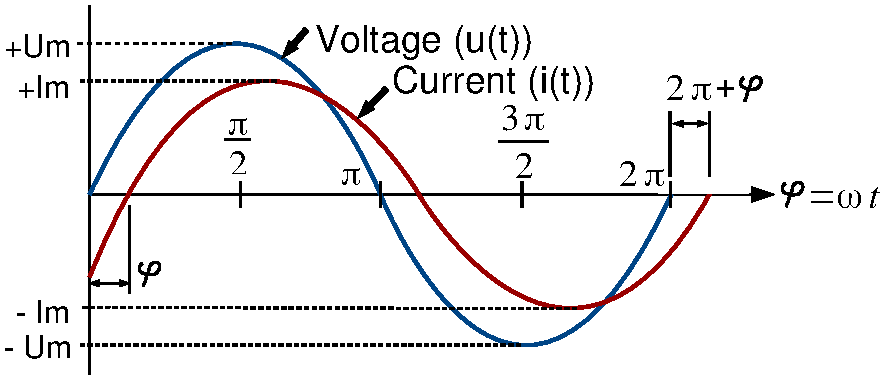
\includegraphics[width=1\linewidth,angle=0]{phase_diff}
\caption{The phase difference between voltage (blue) and current (red), the origin of phase difference of angle $\varphi$}\label{f:ph_diff}
\end{figure}

Considering the figure \ref{f:ph_diff}, the voltage waveform above starts at zero along the horizontal reference axis, but at that same instant of time the current waveform is still negative in value and does not cross this reference axis until 30\degree  later. Then there exists a Phase difference between the two waveforms as the current cross the horizontal reference axis reaching its maximum peak and zero values after the voltage waveform.

As the two waveforms are no longer \textit{in-phase}, they must therefore be \textit{out-of-phase} by an amount determined by phi, $\varphi$. The waveform of the current can also be said to be \textit{lagging} behind the voltage waveform by the phase angle $\varphi$. This angle represents the phase shift (also called phase difference) between two sinusoids \cite{maxfield2011electrical}.


\subsection{Power factor and power factor correction}
The power factor is just a specific name for a phase shift between the sinusoids of a current and voltage. So the figure \ref{f:ph_diff} in fact shows the power factor. However, it is not expressed in a plane angle, but rather as a dimensionless number between -1 and 1.

The power factor is defined as $\frac{P}{S}$, as a ratio of the real power over the apparent power\cite{dixit2010electrical}. If $\varphi$ is the phase angle between the current and voltage, then the power factor is equal to the cosine of the angle, $cos\,\varphi$.

If the power factor is 1, it means that all the supplied power is completely consumed by purely resistive load. A positive power factor that is lower than 1 indicates that some power is not consumed by the load and is returned back. The lower the factor, the more power is returned. When power factor is equal to 0, the energy flow is entirely reactive, and stored energy in the load returns to the source on each cycle. A negative power factor means that the device, considered to be power load is in fact a power source (produces more power than consumes).

How can this information be useful? Every load with a power factor other than 1 returns some power back to the transmission line. Since the transmission lines does have some resistance, this returned power translates to some wasted power in a form of heat. Energetic companies want to minimise the power wasted in the transmission lines to increase their profit, so numerous laws are coming into effect to correct \cite{singh2008electric} (increase) the power factor.



%\subsection{Electric power measurement}
%Measuring the electric power makes most sense on the customer appliances. The first reason is, that they generally consume power that is purchased on contract. The energetic company measures all the power used up by the end customer, but customer has no easy way to see how much and how \textit{effectively} is power used by the appliances. The second important reason is that the appliances has a standardised connector (plug) that is guaranteed to fit in all the area using it, which is not a case for example on battery powered devices (batteries has different sizes, connectors and general properties.
%
%When it comes to measuring the electrical power, the first and the most important thing to discuss is safety. Only after all the safety precautions had been made clear, the theory can be clarified and subsequently, the practice can be applied. 
%
%If not handled with care, operating or manipulating with voltage can cause permanent damage to appliance or health, or can cause fire or even death. Thus, respect, increased care and knowledge is necessary in all further practical steps involved.


\subsection{Power measuring integrated circuits} \label{ss:pmic}

Although it is possible to construct a circuit out of discrete components that would measure \cite{webster2003electrical} the required physical quantities, and such a solution would probably be the cheapest solution out there, it would be highly impractical due to multiple reasons.

The most importantly, the obtained accuracy of the measurements would be dependent on the implementation and used components. It is safe to assume, that without multiple design iterations, the accuracy may be too low to be used in practice.

Another point is that, there is no definitive guide, ready to follow, about how to design such circuit. The reason of this is the vast amount of components available on the market and a lot of design considerations to take into account, depending on the requirements.

A special purpose \glspl{ic} are being developed for the exact purpose of measuring the real, apparent and reactive power, the power factor, and in most cases, gathering some other relevant information.

\begin{figure}[ht!]
\centering
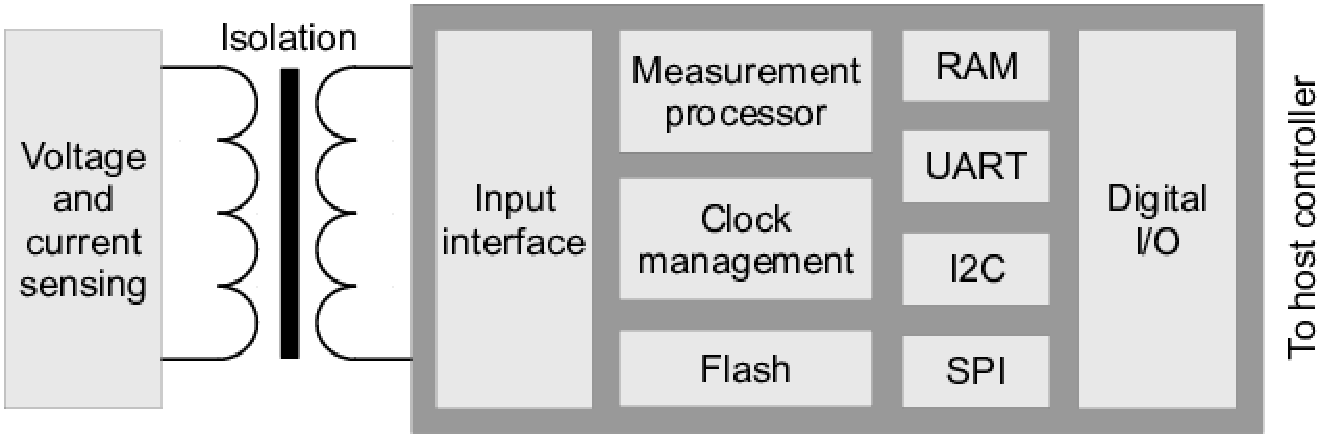
\includegraphics[width=1\linewidth,angle=0]{measurement_IC_diag}
\caption{The simplified block diagram for a power measurement \gls{ic}}\label{f:meas_IC_diag}
\end{figure}

From the block diagram \ref{f:meas_IC_diag}, it can be seen that the power measuring \gls{ic} is just a specialised microcontroller. It takes the data from the sensing circuitry, which in case of voltage can be measured \textit{directly}, provided that the galvanic isolation is included, for the sake of safety. The current however, must be measured \textit{indirectly}. There are three common ways \cite{srinivasan2015composite} of doing so:

\begin{enumerate}
\item \textbf{shunt resistor} - a resistor with a very small but precise value, that causes a voltage drop with a current passing through it due to the Ohm's law, regardless of frequency. The actual voltage drop is so small, that it can be assumed insignificant, but measurable. However, the voltage drop is still present and may cause some issues, if not taken into account. The advantage is really low price. External galvanic isolation must be provided.
\item \textbf{current transformer} - a current passing wire inside a current sensing coil. Since it is a magnetic induction based transformer, the galvanic isolation is naturally present. The disadvantage is, that the transformer has a cut-off frequency, below which it's effect diminishes rapidly. External magnetic fields can cause problems too. Suitable for measuring current of a fixed (or non-decreasing) frequency.
\item \textbf{Hall-effect sensor} - a sensor measuring absolute electromagnetic field in a conductor. In contrast to the current transformer, this sensor is able to measure low frequency currents, down to \gls{dc}, which is a feat that the shunt resistor possesses too. Can be placed anywhere near the current path and doesn't require physical connection, thus providing galvanic isolation too. The price increases with operating currents range and precision. Prone to be disturbed by external magnetic fields, too.
\end{enumerate}

Using dedicated power measuring IC has another advantage apart from being more accurate. In fact, the part \gls{datasheet} can be consulted and if all application notes and advices are abided, the specified accuracy can be guaranteed.



\section{Embedded system}
An embedded \gls{system} is some combination of \gls{computer} \gls{hw} and \gls{sw}, either fixed in capability or programmable, that is specifically designed for a particular function \cite{ganssle2008embedded}. Industrial machines, automobiles, medical equipment, cameras, household appliances, airplanes, vending machines and toys (as well as the more obvious cellular phone and \gls{pda}) are among the myriad possible hosts of an embedded \gls{system}. Embedded \glspl{system} that are programmable are provided with programming \glspl{interface}, and embedded \glspl{system} programming is a specialized occupation.

\subsection{Processing units}
The term embedded \gls{system} is quite broad, so there is no surprise that the spectrum of used processing units is also wide. Since the general purpose microprocessors require external components, namely memories and \glspl{peripheral}, they tend to consume extra power and a board space. Since the design limitations of an embedded \glspl{system} are most of the time low physical size, low power consumption and/or long uptime and ruggedness (more components mean more parts could fail), microprocessors are seldom used. However, most of the commonly used architectures and word lengths are covered. Due to aforementioned reasons, microcontrollers are favored over microprocessors. 

\subsection{ESP8266 Wi-Fi module} \label{s:esp8266}
The ESP8266 Wi-Fi module is a self contained \gls{soc} with integrated \gls{tcpip} protocol stack that can give any microcontroller access to your Wi-Fi network. The ESP8266 is capable of either hosting an application or offloading all Wi-Fi networking functions from another application processor. The ESP8266 module is an extremely cost effective solution, with a huge code-base and community, making it a preferable option for many modern projects, mainly the ones that follow the \gls{iot} trend.

\begin{figure}[ht!]
\centering
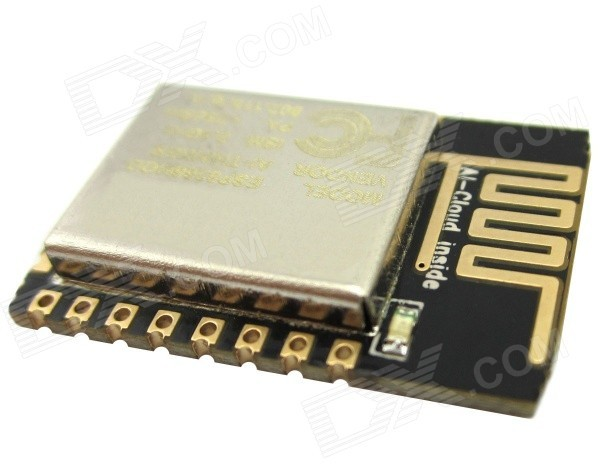
\includegraphics[width=.4\linewidth,angle=0]{esp-12e}
\caption{The certified ESP-12E module exposing all \glspl{gpio}}\label{f:esp-12e}
\end{figure}

This module has a powerful enough on-board processing and storage capability that allows it to be integrated with the sensors and other application specific devices through its \glspl{gpio} with minimal development up-front and minimal loading during runtime. Its high degree of on-chip integration allows for minimal external circuitry, including the front-end module, is designed to occupy minimal \gls{pcb} area. 




\section{Hardware components breakdown} \label{ss:hw}
The device under test will be referred to as \textbf{appliance} and the produced device will be referred to as \textbf{client node} (displayed as a simplified schematic in figure \ref{f:schem_block}) is already integrated as an ESP-8266 module, described in more detail in the chapter \ref{s:esp8266}. The module contains the \gls{tcpip} stack, micro-controller (application processor) running the user program, \gls{wlan} and light indication, all in one piece, so this greatly simplifies the design process and allows for more focus on the actual measurement circuitry. The ESP-12E has been chosen as an actual module, because of the available certification\cite{online:2ADUIESP-12}, which allows it to be introduced to the market later. It was already shown in the figure \ref{f:esp-12e}. The \gls{pwm} is present there too, so sound indication requires just a sound emitting device.

\begin{figure}[ht!]
\centering
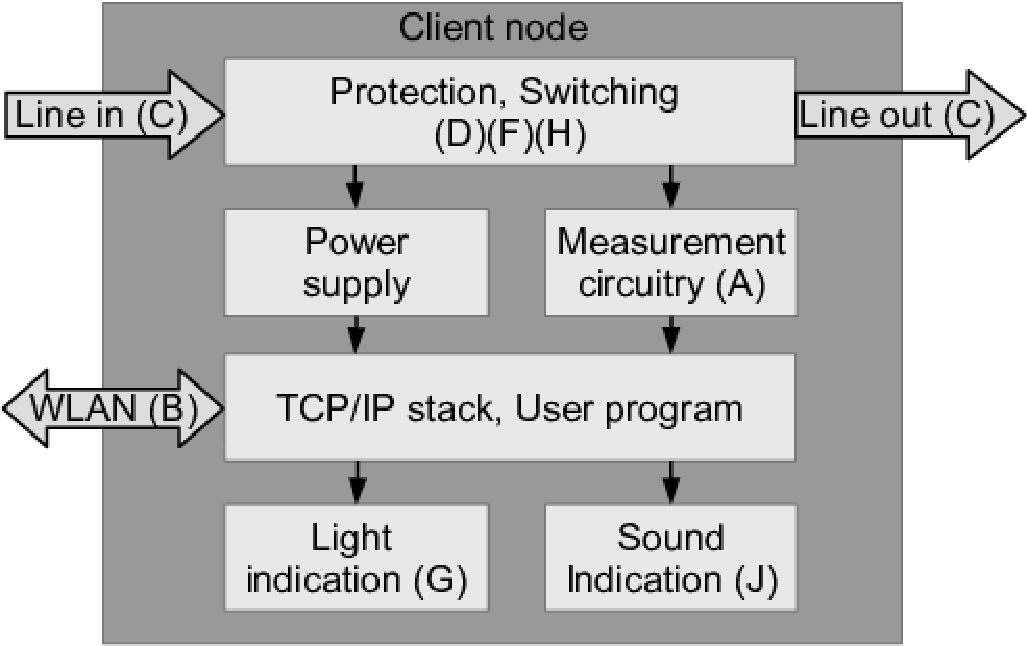
\includegraphics[width=.8\linewidth,angle=0]{client_node_diag}
\caption{The proposed block diagram of a \textit{client node}}\label{f:client_node}
\end{figure}

Talking about the measurement circuitry \ref{f:schem_block}, the viable candidate is MAX78615 \cite{online:MAX78615} with the companion \gls{ic} MAX78700 \cite{online:MAX78700}. The couple should be used, because it provides multiple ways of same voltage level communication with the processor, galvanic isolation via the pulse transformer for improved circuitry protection, great precision, accuracy and utility. The shunt resistor is utilised as a way of obtaining measurements, described in the sub-chapter \ref{ss:pmic}.

For the protection against fire a standard glass fuse or a resettable \gls{ptc} fuse\cite{wright2004electric} should be used. Because of the variable nature of most used devices, it is hard to calculate the current consumption of the circuit. It can be measured after the first iteration is manufactured. Thus, the easily replaceable standard glass fuse has been chosen because of its versatility. The circuit protection against high voltage should be solved with an isolated DC-to-DC converter\cite{carr1996linear} or with a linear transformer coupled with a linear voltage regulator\cite{2008linear}. Since the former one is either expensive or hard to design, and this work does not want to focus on more complexities, the latter option has been chosen.

Choosing the voltage level for the digital electronics (the output voltage of the linear regulator) is straightforward. Since the ESP-12E works on nominal 3.3V, this is the level that has been chosen. Having \glspl{ic} using the same voltage level removes the need to level-shift the communication between them, thus increasing the simplicity of the design.

\begin{figure}[ht!]
\centering
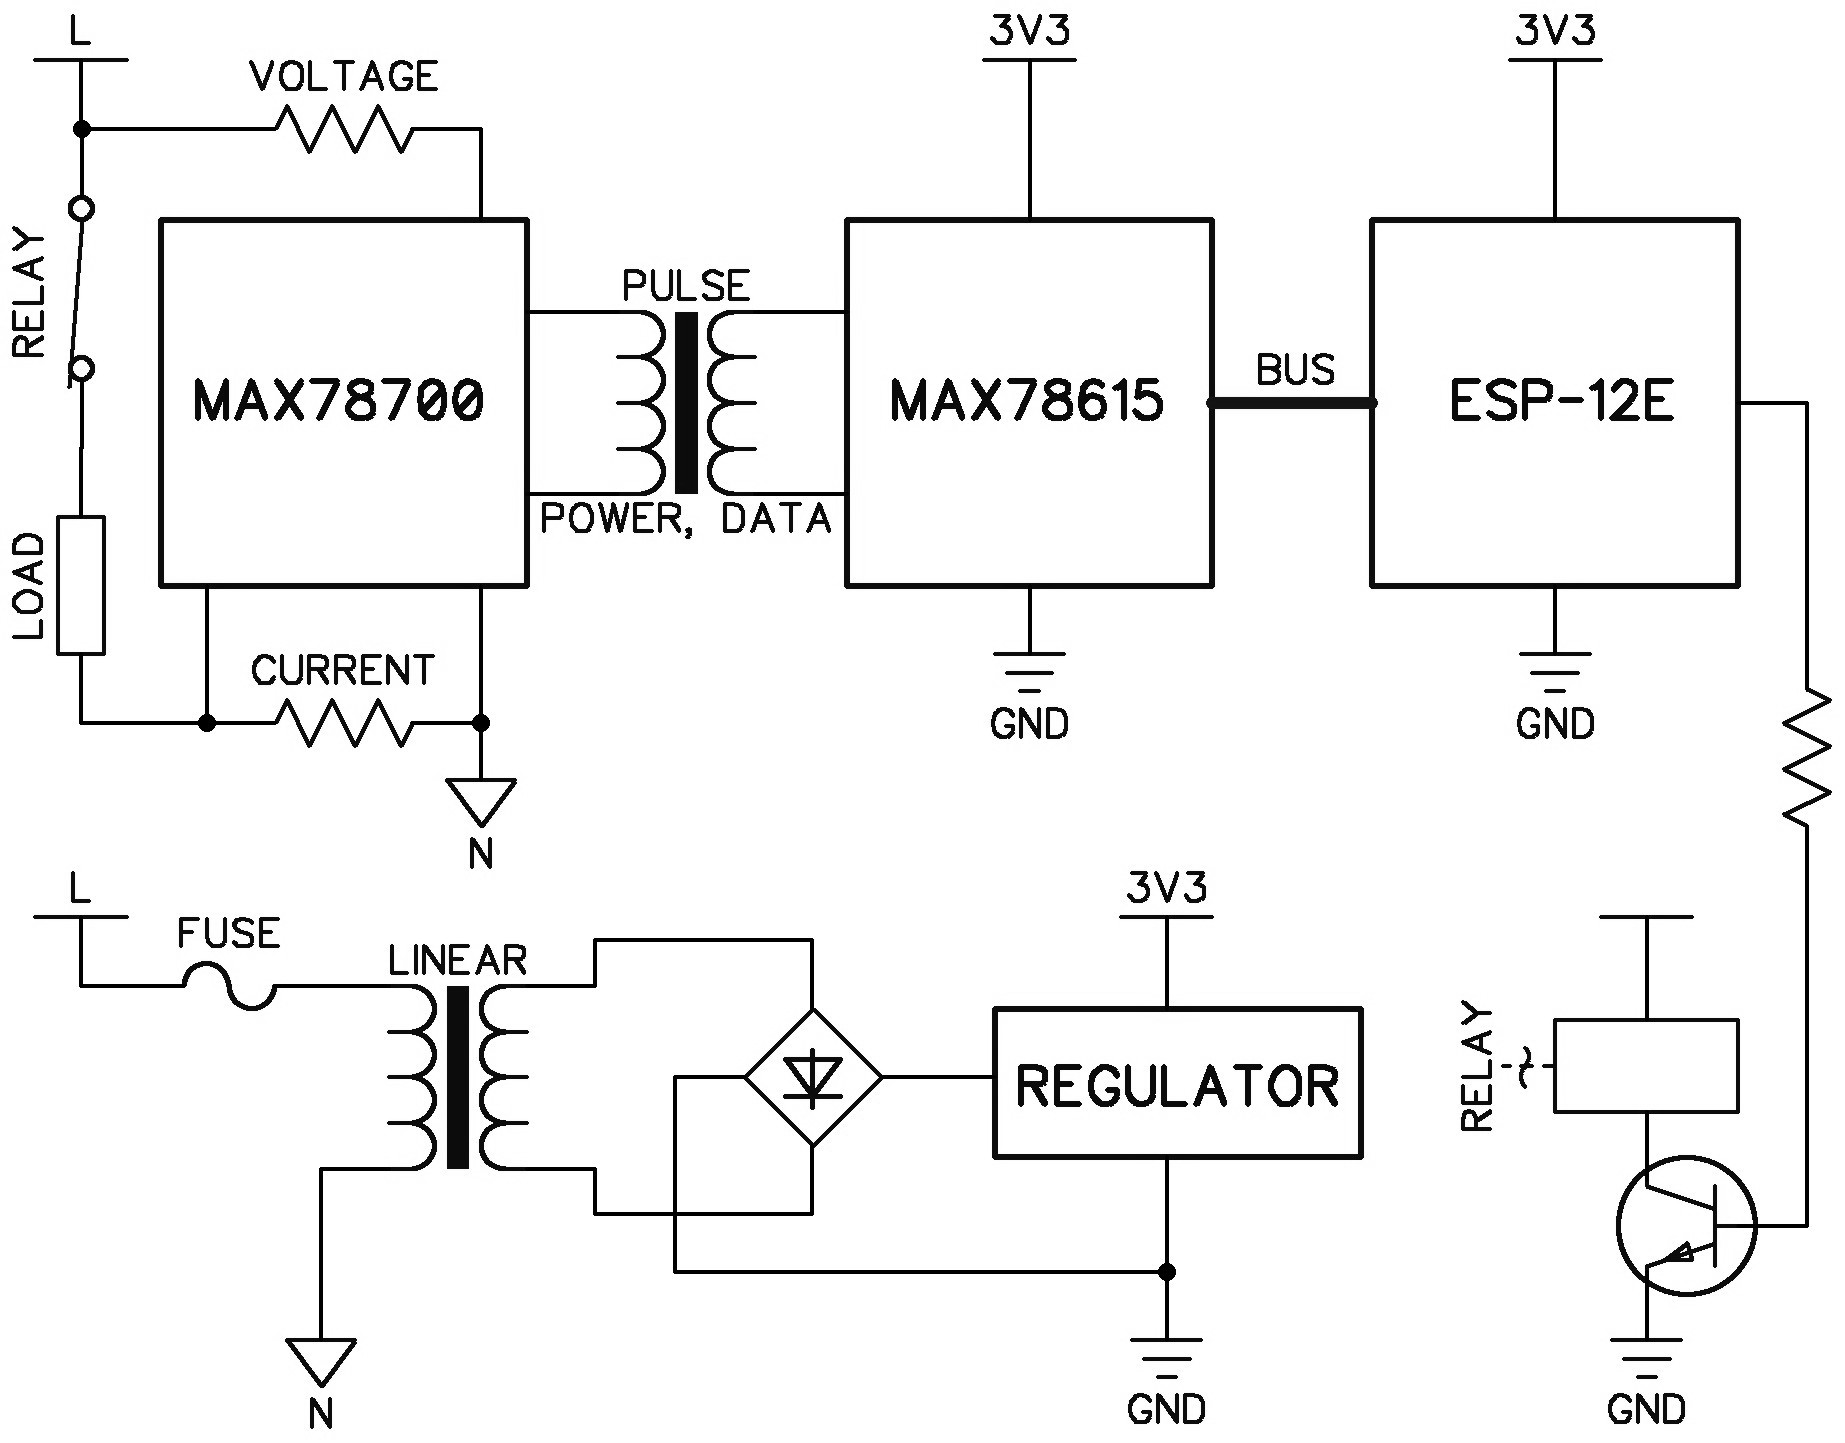
\includegraphics[width=1\linewidth,angle=0]{schematic_block}
\caption{Greatly simplified schematic of a client node sketching the inner working}\label{f:schem_block}
\end{figure}

Talking about the measurement circuitry, the candidate is MAX78615 \cite{online:MAX78615}, working on nominal 3.3V level, along with the companion \gls{ic} MAX78700 \cite{online:MAX78700}. The couple has been chosen, because it provides multiple ways of communication with the processor (buses/serial interfaces), galvanic isolation via a pulse transformer for improved circuitry protection, great precision, accuracy and utility. The resistor network, including the shunt resistor is utilised as a way of obtaining measurements. The shunt resistor is also briefly described in the sub-chapter \ref{ss:pmic}.

The remaining part of the client node's block diagram \ref{f:client_node} not yet mentioned is switching. Either a mechanical relay or a semiconductor device, such as a thyristor or a \gls{ssr} isolated by an opto-coupler\cite{trzynadlowski2015introduction} will do. Mechanical relays tend to be larger and produce sound noise, have slow response time, but have inbuilt separate isolation and are capable of switching higher currents without additional thermal issues than their semiconductor counterparts\cite{blume2008electric}. The disadvantages of the mechanical relay are not relevant here, thus it has been chosen.

\begin{figure}[]
\centering
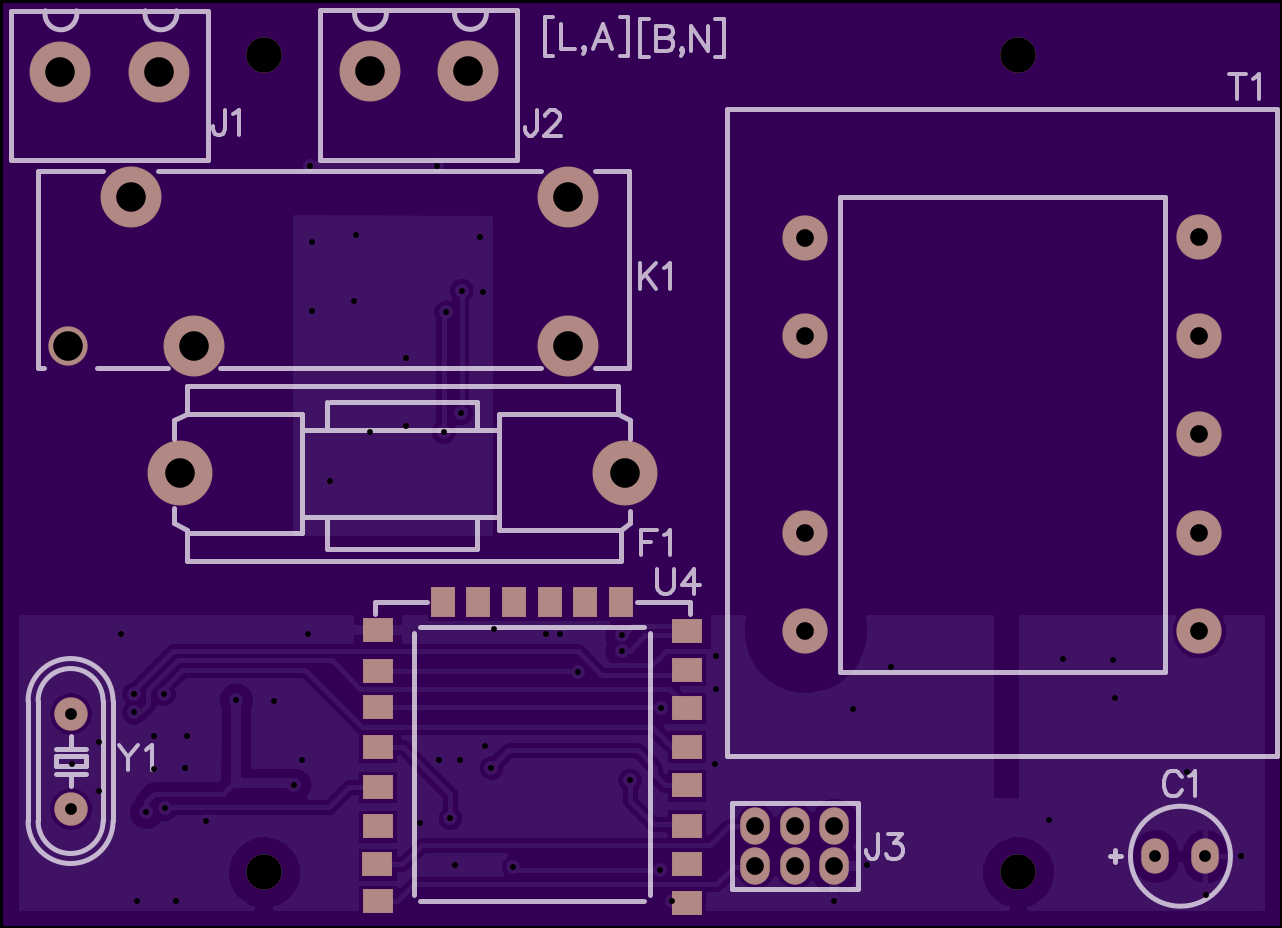
\includegraphics[width=.8\linewidth,angle=0]{pcb_top}
\caption{The top layer of the designed \gls{pcb} (client node), exposing mainy \gls{tht} components}\label{f:pcb_top}
\end{figure}
\begin{figure}[]
\centering
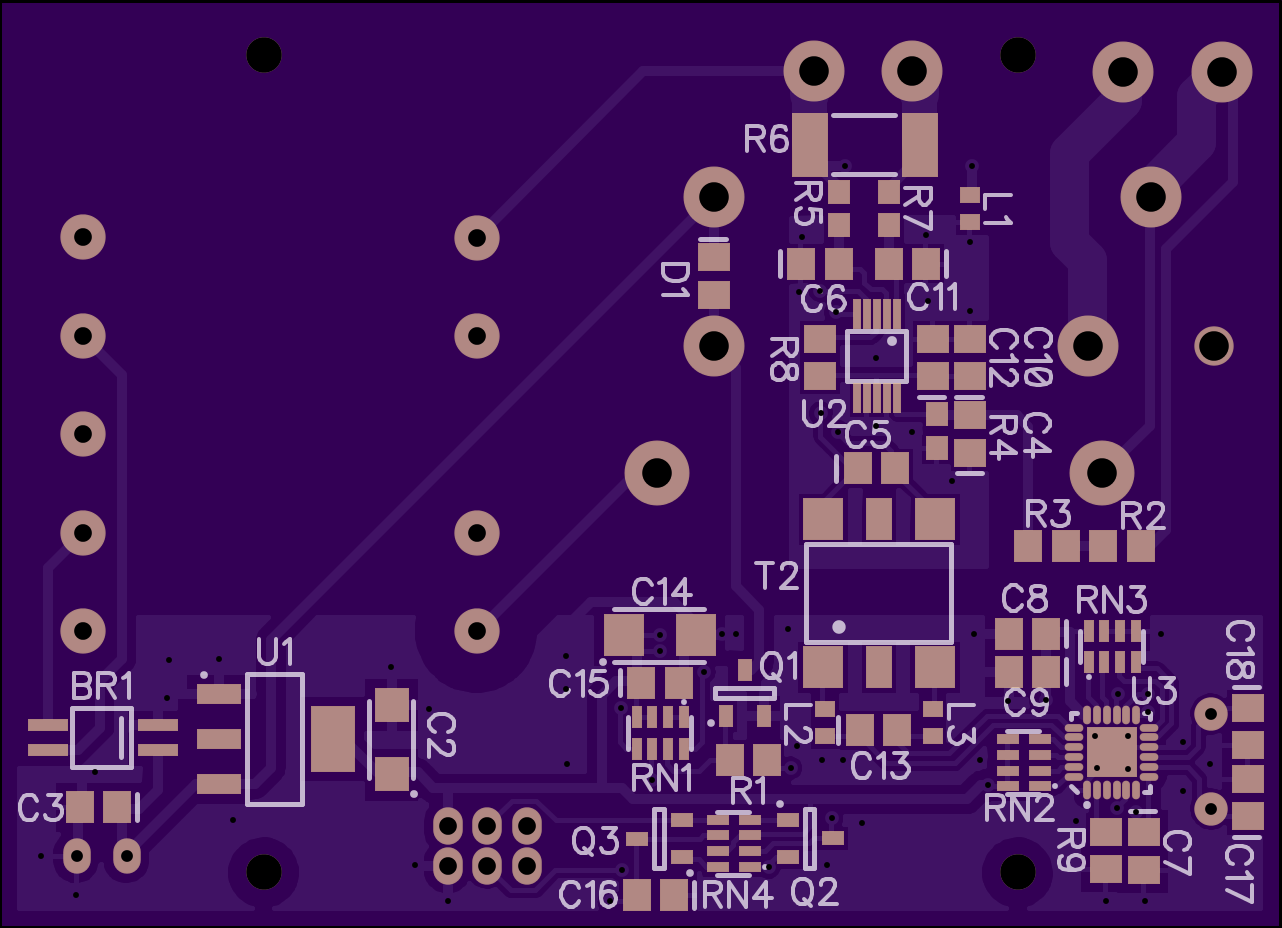
\includegraphics[width=.8\linewidth,angle=0]{pcb_bottom}
\caption{The bottom layer of the designed \gls{pcb} (client node), exposing mainly \gls{smt} components}\label{f:pcb_bottom}
\end{figure}


\section{Conclusion}

The manufactured client node has been inserted into the enclosure\cite{online:enclosure}, portrayed in the figure \ref{f:enclosure}, containing an European mains socket (female) on one side and an European mains plug (male) on the other side, forming a man-in-the-middle adaptor, that can be non-invasively put between wall socket and an appliance. The result can be observed in figure \ref{f:project_inside}.

The client node is capable of measuring \textit{RMS voltage} and \textit{RMS current}. By multiplying them together, the \textit{apparent power} can be obtained, as discussed back in the sub-chapter \ref{ss:power_ac}. The intentions are to fix the design, enabling full range of physical quantities, discussed throughout the chapter \ref{s:el_power}, to be measured. The plan is to use multiple client nodes to measure and track power consumption of the inactive, but plugged-in \gls{smps} chargers, in a form of a collaborative global experiment.

\begin{figure}[]
\centering
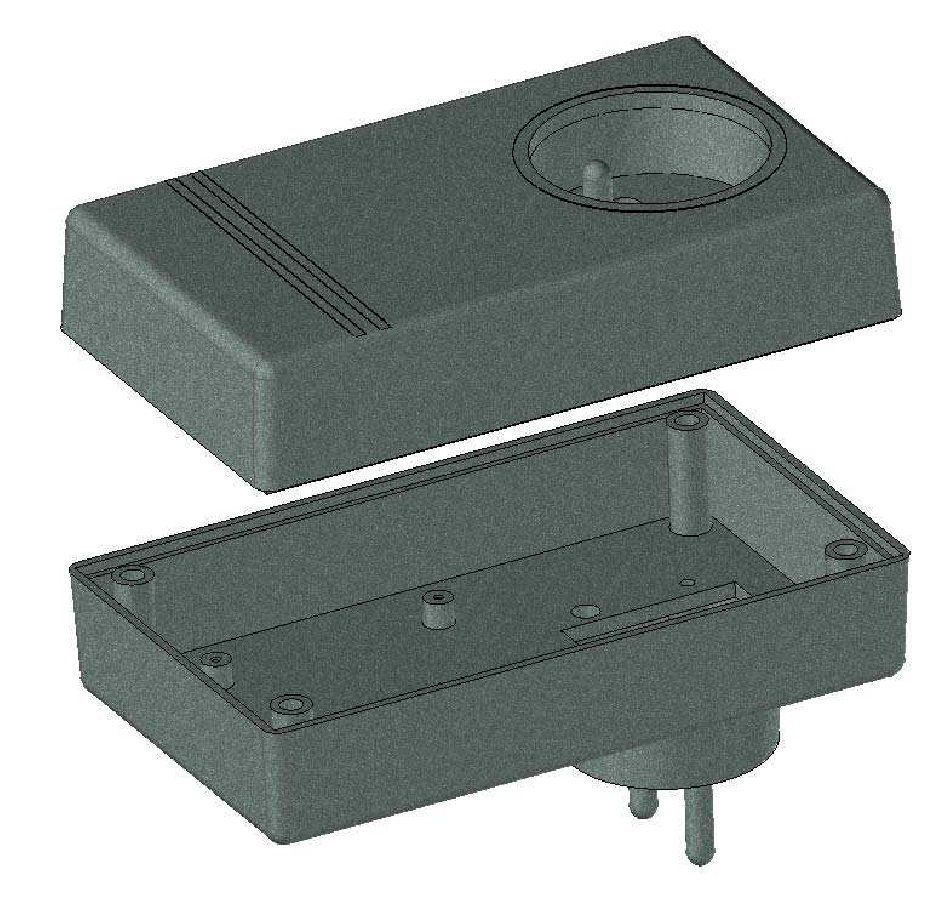
\includegraphics[width=.8\linewidth,angle=0]{enclosure}
\caption{The 3D visualisation of the enclosure, displaying both the plug and the socket}\label{f:enclosure}
\end{figure}
\begin{figure}[]
\centering
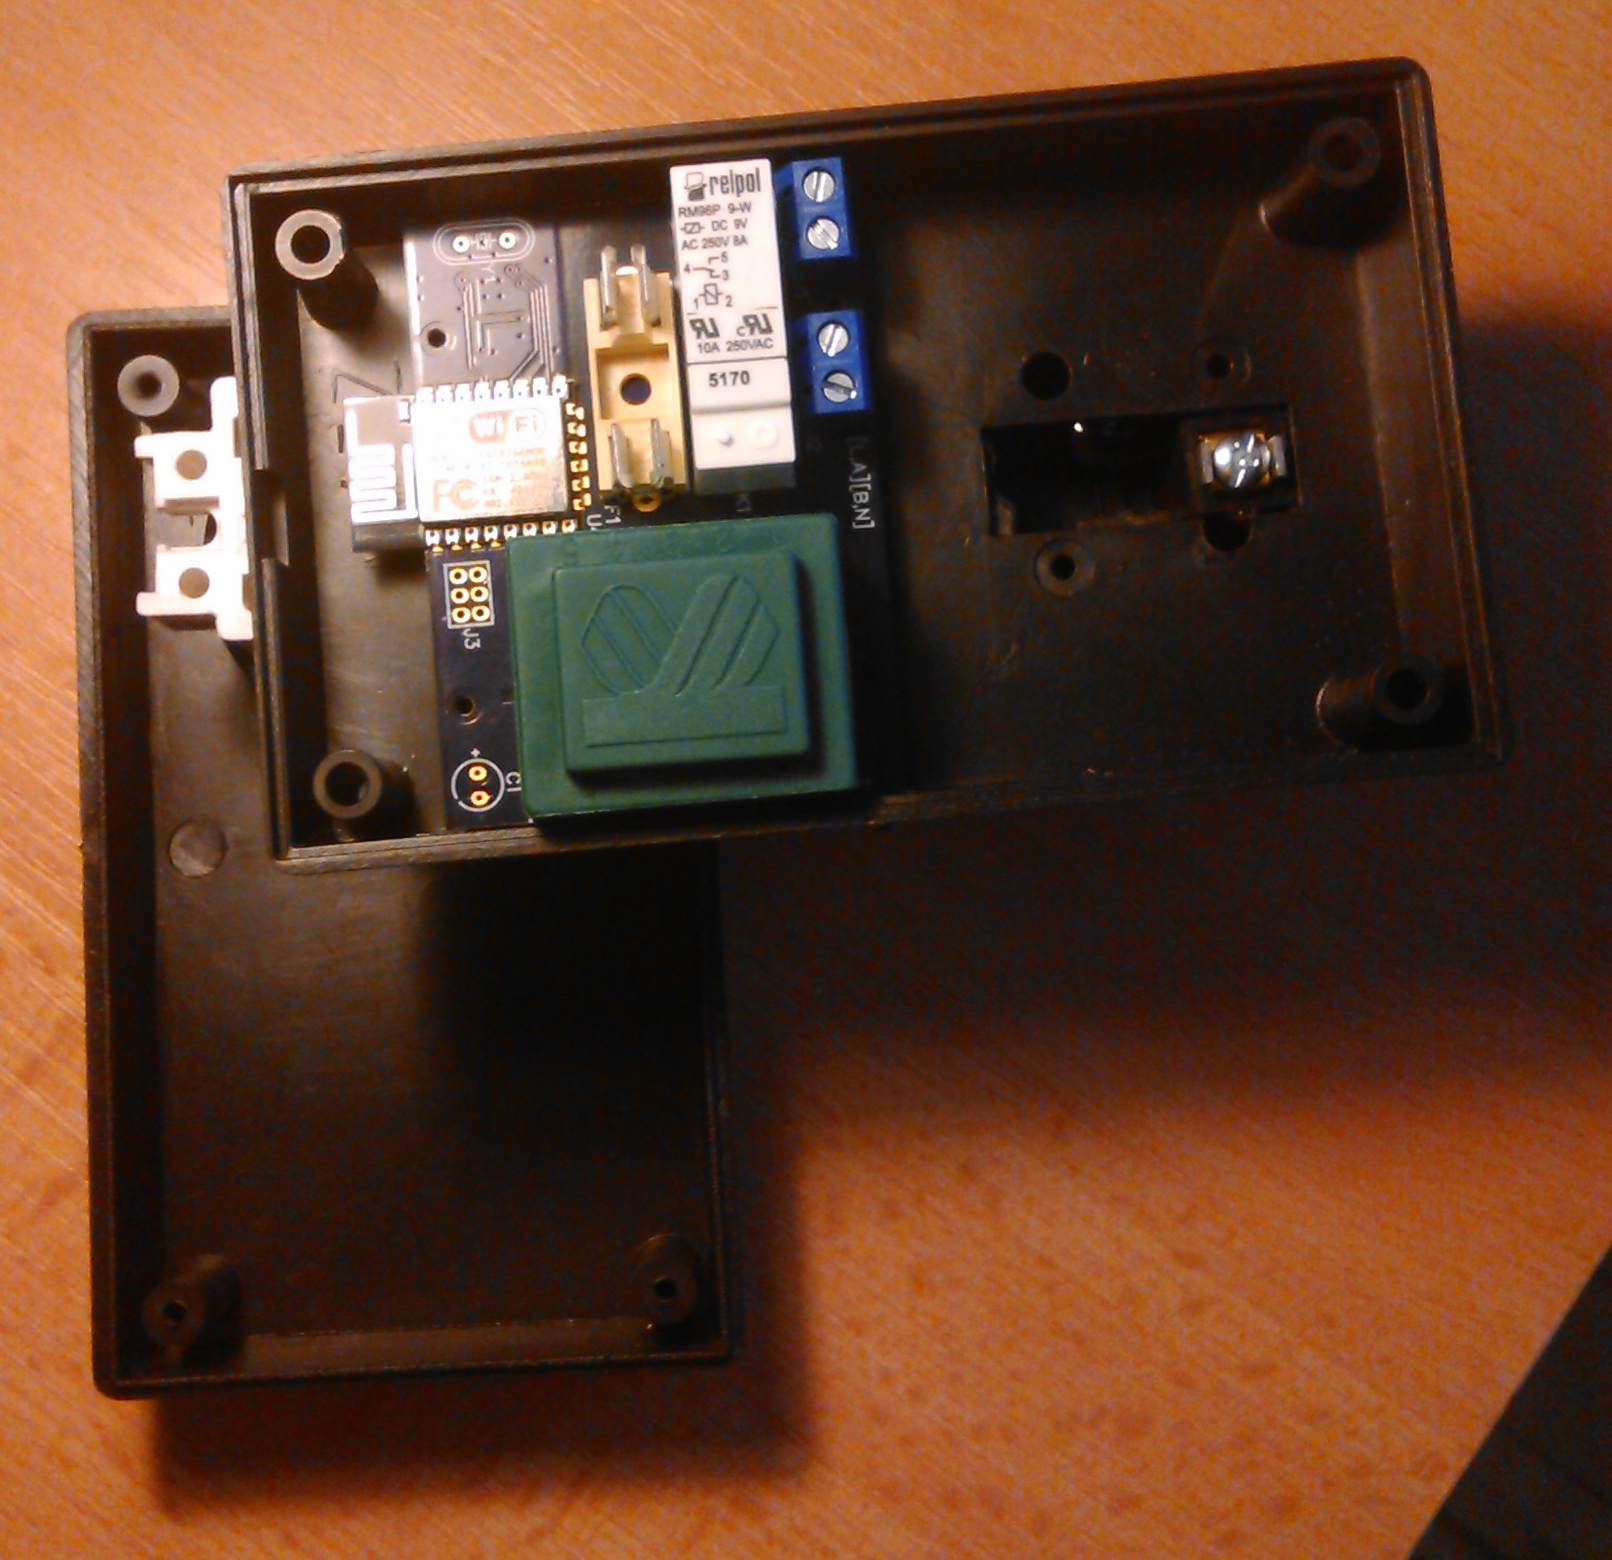
\includegraphics[width=.8\linewidth,angle=0]{project_inside}
\caption{The view into the client node's enclosure, before the final assembly, exposing top side of the board containing linear transformer T1 (green), mains connectors J1 and J2 (blue), a fuse holder for F1 (yellow-ish), a relay K1 (white) and an ESP-12E module}\label{f:project_inside}
\end{figure}


% if have a single appendix:
%\appendix[Proof of the Zonklar Equations]
% or
%\appendix  % for no appendix heading
% do not use \section anymore after \appendix, only \section*
% is possibly needed

% use appendices with more than one appendix
% then use \section to start each appendix
% you must declare a \section before using any
% \subsection or using \label (\appendices by itself
% starts a section numbered zero.)
%


%\appendices
%\section{Proof of the First Zonklar Equation}
%Appendix one text goes here. 
%
%% you can choose not to have a title for an appendix
%% if you want by leaving the argument blank
%\section{}
%Appendix two text goes here.

\newpage
% use section* for acknowledgement
\section*{Acknowledgment}
I would like to express my sincere thanks to my supervisor Ing. Tibor Vince,
PhD., for his constant and constructive guidance throughout all the struggles that
have occurred during this work. And to all other who gave a helping hand, I say
thank you very much, too.


% Can use something like this to put references on a page
% by themselves when using endfloat and the captionsoff option.
%\ifCLASSOPTIONcaptionsoff
%  \newpage
%\fi

\printbibliography



% that's all folks
\end{document}





% An example of a floating figure using the graphicx package.
% Note that \label must occur AFTER (or within) \caption.
% For figures, \caption should occur after the \includegraphics.
% Note that IEEEtran v1.7 and later has special internal code that
% is designed to preserve the operation of \label within \caption
% even when the captionsoff option is in effect. However, because
% of issues like this, it may be the safest practice to put all your
% \label just after \caption rather than within \caption{}.
%
% Reminder: the "draftcls" or "draftclsnofoot", not "draft", class
% option should be used if it is desired that the figures are to be
% displayed while in draft mode.
%
%\begin{figure}[!t]
%\centering
%\includegraphics[width=2.5in]{myfigure}
% where an .eps filename suffix will be assumed under latex, 
% and a .pdf suffix will be assumed for pdflatex; or what has been declared
% via \DeclareGraphicsExtensions.
%\caption{Simulation Results.}
%\label{fig_sim}
%\end{figure}

% Note that IEEE typically puts floats only at the top, even when this
% results in a large percentage of a column being occupied by floats.


% An example of a double column floating figure using two subfigures.
% (The subfig.sty package must be loaded for this to work.)
% The subfigure \label commands are set within each subfloat command,
% and the \label for the overall figure must come after \caption.
% \hfil is used as a separator to get equal spacing.
% Watch out that the combined width of all the subfigures on a 
% line do not exceed the text width or a line break will occur.
%
%\begin{figure*}[!t]
%\centering
%\subfloat[Case I]{\includegraphics[width=2.5in]{box}%
%\label{fig_first_case}}
%\hfil
%\subfloat[Case II]{\includegraphics[width=2.5in]{box}%
%\label{fig_second_case}}
%\caption{Simulation results.}
%\label{fig_sim}
%\end{figure*}
%
% Note that often IEEE papers with subfigures do not employ subfigure
% captions (using the optional argument to \subfloat[]), but instead will
% reference/describe all of them (a), (b), etc., within the main caption.


% An example of a floating table. Note that, for IEEE style tables, the 
% \caption command should come BEFORE the table. Table text will default to
% \footnotesize as IEEE normally uses this smaller font for tables.
% The \label must come after \caption as always.
%
%\begin{table}[!t]
%% increase table row spacing, adjust to taste
%\renewcommand{\arraystretch}{1.3}
% if using array.sty, it might be a good idea to tweak the value of
% \extrarowheight as needed to properly center the text within the cells
%\caption{An Example of a Table}
%\label{table_example}
%\centering
%% Some packages, such as MDW tools, offer better commands for making tables
%% than the plain LaTeX2e tabular which is used here.
%\begin{tabular}{|c||c|}
%\hline
%One & Two\\
%\hline
%Three & Four\\
%\hline
%\end{tabular}
%\end{table}


% Note that IEEE does not put floats in the very first column - or typically
% anywhere on the first page for that matter. Also, in-text middle ("here")
% positioning is not used. Most IEEE journals use top floats exclusively.
% Note that, LaTeX2e, unlike IEEE journals, places footnotes above bottom
% floats. This can be corrected via the \fnbelowfloat command of the
% stfloats package.




% Some very useful LaTeX packages include:
% (uncomment the ones you want to load)


% *** MISC UTILITY PACKAGES ***
%
%\usepackage{ifpdf}
% Heiko Oberdiek's ifpdf.sty is very useful if you need conditional
% compilation based on whether the output is pdf or dvi.
% usage:
% \ifpdf
%   % pdf code
% \else
%   % dvi code
% \fi
% The latest version of ifpdf.sty can be obtained from:
% http://www.ctan.org/tex-archive/macros/latex/contrib/oberdiek/
% Also, note that IEEEtran.cls V1.7 and later provides a builtin
% \ifCLASSINFOpdf conditional that works the same way.
% When switching from latex to pdflatex and vice-versa, the compiler may
% have to be run twice to clear warning/error messages.






% *** CITATION PACKAGES ***
%
%\usepackage{cite}
% cite.sty was written by Donald Arseneau
% V1.6 and later of IEEEtran pre-defines the format of the cite.sty package
% \cite{} output to follow that of IEEE. Loading the cite package will
% result in citation numbers being automatically sorted and properly
% "compressed/ranged". e.g., [1], [9], [2], [7], [5], [6] without using
% cite.sty will become [1], [2], [5]--[7], [9] using cite.sty. cite.sty's
% \cite will automatically add leading space, if needed. Use cite.sty's
% noadjust option (cite.sty V3.8 and later) if you want to turn this off
% such as if a citation ever needs to be enclosed in parenthesis.
% cite.sty is already installed on most LaTeX systems. Be sure and use
% version 4.0 (2003-05-27) and later if using hyperref.sty. cite.sty does
% not currently provide for hyperlinked citations.
% The latest version can be obtained at:
% http://www.ctan.org/tex-archive/macros/latex/contrib/cite/
% The documentation is contained in the cite.sty file itself.






% *** MATH PACKAGES ***
%
%\usepackage[cmex10]{amsmath}
% A popular package from the American Mathematical Society that provides
% many useful and powerful commands for dealing with mathematics. If using
% it, be sure to load this package with the cmex10 option to ensure that
% only type 1 fonts will utilized at all point sizes. Without this option,
% it is possible that some math symbols, particularly those within
% footnotes, will be rendered in bitmap form which will result in a
% document that can not be IEEE Xplore compliant!
%
% Also, note that the amsmath package sets \interdisplaylinepenalty to 10000
% thus preventing page breaks from occurring within multiline equations. Use:
%\interdisplaylinepenalty=2500
% after loading amsmath to restore such page breaks as IEEEtran.cls normally
% does. amsmath.sty is already installed on most LaTeX systems. The latest
% version and documentation can be obtained at:
% http://www.ctan.org/tex-archive/macros/latex/required/amslatex/math/





% *** SPECIALIZED LIST PACKAGES ***
%
%\usepackage{algorithmic}
% algorithmic.sty was written by Peter Williams and Rogerio Brito.
% This package provides an algorithmic environment fo describing algorithms.
% You can use the algorithmic environment in-text or within a figure
% environment to provide for a floating algorithm. Do NOT use the algorithm
% floating environment provided by algorithm.sty (by the same authors) or
% algorithm2e.sty (by Christophe Fiorio) as IEEE does not use dedicated
% algorithm float types and packages that provide these will not provide
% correct IEEE style captions. The latest version and documentation of
% algorithmic.sty can be obtained at:
% http://www.ctan.org/tex-archive/macros/latex/contrib/algorithms/
% There is also a support site at:
% http://algorithms.berlios.de/index.html
% Also of interest may be the (relatively newer and more customizable)
% algorithmicx.sty package by Szasz Janos:
% http://www.ctan.org/tex-archive/macros/latex/contrib/algorithmicx/




% *** ALIGNMENT PACKAGES ***
%
%\usepackage{array}
% Frank Mittelbach's and David Carlisle's array.sty patches and improves
% the standard LaTeX2e array and tabular environments to provide better
% appearance and additional user controls. As the default LaTeX2e table
% generation code is lacking to the point of almost being broken with
% respect to the quality of the end results, all users are strongly
% advised to use an enhanced (at the very least that provided by array.sty)
% set of table tools. array.sty is already installed on most systems. The
% latest version and documentation can be obtained at:
% http://www.ctan.org/tex-archive/macros/latex/required/tools/


% IEEEtran contains the IEEEeqnarray family of commands that can be used to
% generate multiline equations as well as matrices, tables, etc., of high
% quality.




% *** SUBFIGURE PACKAGES ***
%\ifCLASSOPTIONcompsoc
%  \usepackage[caption=false,font=normalsize,labelfont=sf,textfont=sf]{subfig}
%\else
%  \usepackage[caption=false,font=footnotesize]{subfig}
%\fi
% subfig.sty, written by Steven Douglas Cochran, is the modern replacement
% for subfigure.sty, the latter of which is no longer maintained and is
% incompatible with some LaTeX packages including fixltx2e. However,
% subfig.sty requires and automatically loads Axel Sommerfeldt's caption.sty
% which will override IEEEtran.cls' handling of captions and this will result
% in non-IEEE style figure/table captions. To prevent this problem, be sure
% and invoke subfig.sty's "caption=false" package option (available since
% subfig.sty version 1.3, 2005/06/28) as this is will preserve IEEEtran.cls
% handling of captions.
% Note that the Computer Society format requires a larger sans serif font
% than the serif footnote size font used in traditional IEEE formatting
% and thus the need to invoke different subfig.sty package options depending
% on whether compsoc mode has been enabled.
%
% The latest version and documentation of subfig.sty can be obtained at:
% http://www.ctan.org/tex-archive/macros/latex/contrib/subfig/




% *** FLOAT PACKAGES ***
%
%\usepackage{fixltx2e}
% fixltx2e, the successor to the earlier fix2col.sty, was written by
% Frank Mittelbach and David Carlisle. This package corrects a few problems
% in the LaTeX2e kernel, the most notable of which is that in current
% LaTeX2e releases, the ordering of single and double column floats is not
% guaranteed to be preserved. Thus, an unpatched LaTeX2e can allow a
% single column figure to be placed prior to an earlier double column
% figure. The latest version and documentation can be found at:
% http://www.ctan.org/tex-archive/macros/latex/base/


%\usepackage{stfloats}
% stfloats.sty was written by Sigitas Tolusis. This package gives LaTeX2e
% the ability to do double column floats at the bottom of the page as well
% as the top. (e.g., "\begin{figure*}[!b]" is not normally possible in
% LaTeX2e). It also provides a command:
%\fnbelowfloat
% to enable the placement of footnotes below bottom floats (the standard
% LaTeX2e kernel puts them above bottom floats). This is an invasive package
% which rewrites many portions of the LaTeX2e float routines. It may not work
% with other packages that modify the LaTeX2e float routines. The latest
% version and documentation can be obtained at:
% http://www.ctan.org/tex-archive/macros/latex/contrib/sttools/
% Do not use the stfloats baselinefloat ability as IEEE does not allow
% \baselineskip to stretch. Authors submitting work to the IEEE should note
% that IEEE rarely uses double column equations and that authors should try
% to avoid such use. Do not be tempted to use the cuted.sty or midfloat.sty
% packages (also by Sigitas Tolusis) as IEEE does not format its papers in
% such ways.
% Do not attempt to use stfloats with fixltx2e as they are incompatible.
% Instead, use Morten Hogholm'a dblfloatfix which combines the features
% of both fixltx2e and stfloats:
%
% \usepackage{dblfloatfix}
% The latest version can be found at:
% http://www.ctan.org/tex-archive/macros/latex/contrib/dblfloatfix/




%\ifCLASSOPTIONcaptionsoff
%  \usepackage[nomarkers]{endfloat}
% \let\MYoriglatexcaption\caption
% \renewcommand{\caption}[2][\relax]{\MYoriglatexcaption[#2]{#2}}
%\fi
% endfloat.sty was written by James Darrell McCauley, Jeff Goldberg and 
% Axel Sommerfeldt. This package may be useful when used in conjunction with 
% IEEEtran.cls'  captionsoff option. Some IEEE journals/societies require that
% submissions have lists of figures/tables at the end of the paper and that
% figures/tables without any captions are placed on a page by themselves at
% the end of the document. If needed, the draftcls IEEEtran class option or
% \CLASSINPUTbaselinestretch interface can be used to increase the line
% spacing as well. Be sure and use the nomarkers option of endfloat to
% prevent endfloat from "marking" where the figures would have been placed
% in the text. The two hack lines of code above are a slight modification of
% that suggested by in the endfloat docs (section 8.4.1) to ensure that
% the full captions always appear in the list of figures/tables - even if
% the user used the short optional argument of \caption[]{}.
% IEEE papers do not typically make use of \caption[]'s optional argument,
% so this should not be an issue. A similar trick can be used to disable
% captions of packages such as subfig.sty that lack options to turn off
% the subcaptions:
% For subfig.sty:
% \let\MYorigsubfloat\subfloat
% \renewcommand{\subfloat}[2][\relax]{\MYorigsubfloat[]{#2}}
% However, the above trick will not work if both optional arguments of
% the \subfloat command are used. Furthermore, there needs to be a
% description of each subfigure *somewhere* and endfloat does not add
% subfigure captions to its list of figures. Thus, the best approach is to
% avoid the use of subfigure captions (many IEEE journals avoid them anyway)
% and instead reference/explain all the subfigures within the main caption.
% The latest version of endfloat.sty and its documentation can obtained at:
% http://www.ctan.org/tex-archive/macros/latex/contrib/endfloat/
%
% The IEEEtran \ifCLASSOPTIONcaptionsoff conditional can also be used
% later in the document, say, to conditionally put the References on a 
% page by themselves.




% *** PDF, URL AND HYPERLINK PACKAGES ***
%
%\usepackage{url}
% url.sty was written by Donald Arseneau. It provides better support for
% handling and breaking URLs. url.sty is already installed on most LaTeX
% systems. The latest version and documentation can be obtained at:
% http://www.ctan.org/tex-archive/macros/latex/contrib/url/
% Basically, \url{my_url_here}.







% trigger a \newpage just before the given reference
% number - used to balance the columns on the last page
% adjust value as needed - may need to be readjusted if
% the document is modified later
%\IEEEtriggeratref{8}
% The "triggered" command can be changed if desired:
%\IEEEtriggercmd{\enlargethispage{-5in}}

% references section

% can use a bibliography generated by BibTeX as a .bbl file
% BibTeX documentation can be easily obtained at:
% http://www.ctan.org/tex-archive/biblio/bibtex/contrib/doc/
% The IEEEtran BibTeX style support page is at:
% http://www.michaelshell.org/tex/ieeetran/bibtex/
% argument is your BibTeX string definitions and bibliography database(s)
%\bibliographystyle{IEEEtran}
%\bibliography{IEEEabrv,electrical}
%\pagebreak

% <OR> manually copy in the resultant .bbl file
% set second argument of \begin to the number of references
% (used to reserve space for the reference number labels box)
%\begin{thebibliography}{1}
%
%\bibitem{IEEEhowto:kopka}
%H.~Kopka and P.~W. Daly, \emph{A Guide to \LaTeX}, 3rd~ed.\hskip 1em plus
%  0.5em minus 0.4em\relax Harlow, England: Addison-Wesley, 1999.
%
%\end{thebibliography}

% biography section
% 
% If you have an EPS/PDF photo (graphicx package needed) extra braces are
% needed around the contents of the optional argument to biography to prevent
% the LaTeX parser from getting confused when it sees the complicated
% \includegraphics command within an optional argument. (You could create
% your own custom macro containing the \includegraphics command to make things
% simpler here.)
%\begin{IEEEbiography}[{\includegraphics[width=1in,height=1.25in,clip,keepaspectratio]{mshell}}]{Michael Shell}
% or if you just want to reserve a space for a photo:

%\begin{IEEEbiography}{Michael Shell}
%Biography text here.
%\end{IEEEbiography}

% if you will not have a photo at all:
%\begin{IEEEbiographynophoto}{John Doe}
%Biography text here.
%\end{IEEEbiographynophoto}

% insert where needed to balance the two columns on the last page with
% biographies
%\newpage

%\begin{IEEEbiographynophoto}{Jane Doe}
%Biography text here.
%\end{IEEEbiographynophoto}

% You can push biographies down or up by placing
% a \vfill before or after them. The appropriate
% use of \vfill depends on what kind of text is
% on the last page and whether or not the columns
% are being equalized.

%\vfill

% Can be used to pull up biographies so that the bottom of the last one
% is flush with the other column.
%\enlargethispage{-5in}
